\chapter{Introduction}

\section{Welcome}
	Welcome to the $\labview$ course, for 3rd year physics students, at UJ.\\
	In your first semester of $3^{rd}$ year, you have been exposed to a programming language called \texttt{C++}, an \textit{Object-Oriented} text based computer language.\\
	With this mighty tool in hand, you made a little microcontroller do your bidding, specifically an \texttt{ATmega328} found on the Arduino boards.\\
	
	You may have noticed how terse statements in \texttt{C++} can get, sometimes obfuscating the programmers intent, see listing \ref{tinychess} on page \pageref{tinychess} for an extreme example. In this course however, we will not be dealing with text based statements, instead you will make a computer bend to your will by means of pictures and threads!\\
	
	Before we jump into the details, let us first compare two programs performing the same task, one written in \texttt{C}, and one assembled in \texttt{LabVIEW}.\\
	Suppose we want to capture two decimal numbers from a user in order to compute the sum of said numbers:
	
	\subsubsection{C Programming}
	In listing \ref{Ccode}, on page \pageref{Ccode}, the first line imports the required libraries for \texttt{C} to handle our input and output, or \texttt{IO}. We then have to declare what type of variables we are storing and give them names, in this case \texttt{numberA \& numberB}. In this case, the values are initialised to $0$, not required for this example, but good practice regardless. The numbers are then captured from the user on line 7 \& 8. Finally, the results are printed so that the user may see that their system can indeed do basic arithmetic.
	\begin{lstlisting}[language=C, caption=This listing is executable C code see http://www.nanochess.org, label=tinychess,float]
	char*l="ustvrtsuqqqqqqqqyyyyyyyy}{|~z|{}"
	"   76Lsabcddcba .pknbrq  PKNBRQ ?A6J57IKJT576,+-48HLSU";
	#define F getchar()&z
	#define v X(0,0,0,21,
	#define Z while(
	#define _ ;if(
	#define P return--G,y^=8,
	B,i,y,u,b,I[411],*G=I,x=10,z=15,M=1e4;X(w,c,h,e,S,s){int t,o,L,E,d,O=e,N=-M*M,K
	=78-h<<x,p,*g,n,*m,A,q,r,C,J,a=y?-x:x;y^=8;G++;d=w||s&&s>=h&&v 0,0)>M;do{_ o=I[
	p=O]){q=o&z^y _ q<7){A=q--&2?8:4;C=o-9&z?q["& .$  "]:42;do{r=I[p+=C[l]-64]_!w|p
	==w){g=q|p+a-S?0:I+S _!r&(q|A<3||g)||(r+1&z^y)>9&&q|A>2){_ m=!(r-2&7))P G[1]=O,
	K;J=n=o&z;E=I[p-a]&z;t=q|E-7?n:(n+=2,6^y);Z n<=t){L=r?l[r&7]*9-189-h-q:0 _ s)L
	+=(1-q?l[p/x+5]-l[O/x+5]+l[p%x+6]*-~!q-l[O%x+6]+o/16*8:!!m*9)+(q?0:!(I[p-1]^n)+
	!(I[p+1]^n)+l[n&7]*9-386+!!g*99+(A<2))+!(E^y^9)_ s>h||1<s&s==h&&L>z|d){p[I]=n,O
	[I]=m?*g=*m,*m=0:g?*g=0:0;L-=X(s>h|d?0:p,L-N,h+1,G[1],J=q|A>1?0:p,s)_!(h||s-1|B
	-O|i-n|p-b|L<-M))P y^=8,u=J;J=q-1|A<7||m||!s|d|r|o<z||v 0,0)>M;O[I]=o;p[I]=r;m?
	*m=*g,*g=0:g?*g=9^y:0;}_ L>N){*G=O _ s>1){_ h&&c-L<0)P L _!h)i=n,B=O,b=p;}N=L;}
	n+=J||(g=I+p,m=p<O?g-3:g+2,*m<z|m[O-p]||I[p+=p-O]);}}}}Z!r&q>2||(p=O,q|A>2|o>z&
	!r&&++C*--A));}}}Z++O>98?O=20:e-O);P N+M*M&&N>-K+1924|d?N:0;}main(){Z++B<121)*G
	++=B/x%x<2|B%x<2?7:B/x&4?0:*l++&31;Z B=19){Z B++<99)putchar(B%x?l[B[I]|16]:x)_
	x-(B=F)){i=I[B+=(x-F)*x]&z;b=F;b+=(x-F)*x;Z x-(*G=F))i=*G^8^y;}else v u,5);v u,
	1);}}
	\end{lstlisting}
	\begin{lstlisting}[language=C, caption=A simple C program to add two user typed numbers, label=Ccode, float]
	#include<stdio.h>
	
	int main() {
		
		double numberA = 0;
		double numberB = 0;
		scanf("%f", &numberA);
		scanf("%f", &numberB);
		
		printf("%d + %d = ",numberA, numberB, numberA + numberB);
		return 0;
	}
\end{lstlisting}

	\subsubsection{LabVIEW Programming}
	Without having any idea what $\labview$ is, I am sure you are able to follow what figure \ref{Labview1}, on page \pageref{Labview1}, is attempting to convey. In figure \ref{GUI1}  you will find the \textit{Graphical User Interface}, or GUI, for the summing program. The two figures are one program developed simultaneously, we will dive into the details throughout the course.\\
	
	Before you even ask, yes it is really that simple. You will find that creating programs in $\labview$ is fun and rewarding, so relax and take it easy. By the end of this course, you will be able to create complex programs to help you solve problems in physics, as well as bridge the gap between the computer world and the real world.
	\begin{figure}
		\centering
		\begin{subfigure}[b]{0.49\textwidth}
			\centering
			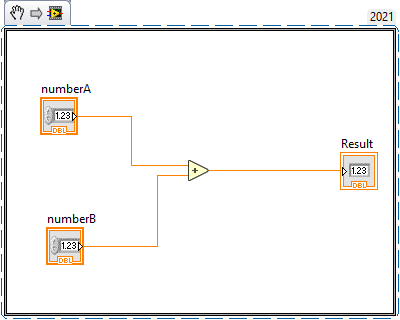
\includegraphics[width=\textwidth]{Labview1}
			\caption{A $\labview$ block diagram.}
			\label{Labview1}
		\end{subfigure}
	\hfill
		\begin{subfigure}[b]{0.49\textwidth}
			\centering
			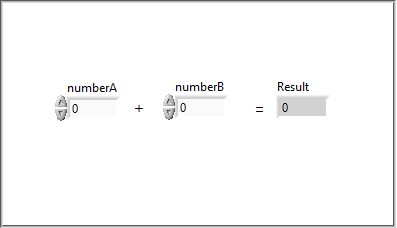
\includegraphics[width=\textwidth]{GUI1}
			\caption{A $\labview$ front panel.}
			\label{GUI1}
	\end{subfigure}
		\caption{A $\labview$ program to sum two numbers.}
		\label{Labview1s}
	\end{figure}

	\section{The LabVIEW Interface}
	\subsection{Introduction}
	$\labview$ usually greats you with a launcher, figure \ref{startup}. From here you may open your recent projects, start a fresh project, or open a virtual instrument, known as a VI. For now, from the ``File'' drop down menu, select ``New VI'' or press \texttt{Ctrl+N} on your keyboard.\\
	\begin{figure}
		\centering
		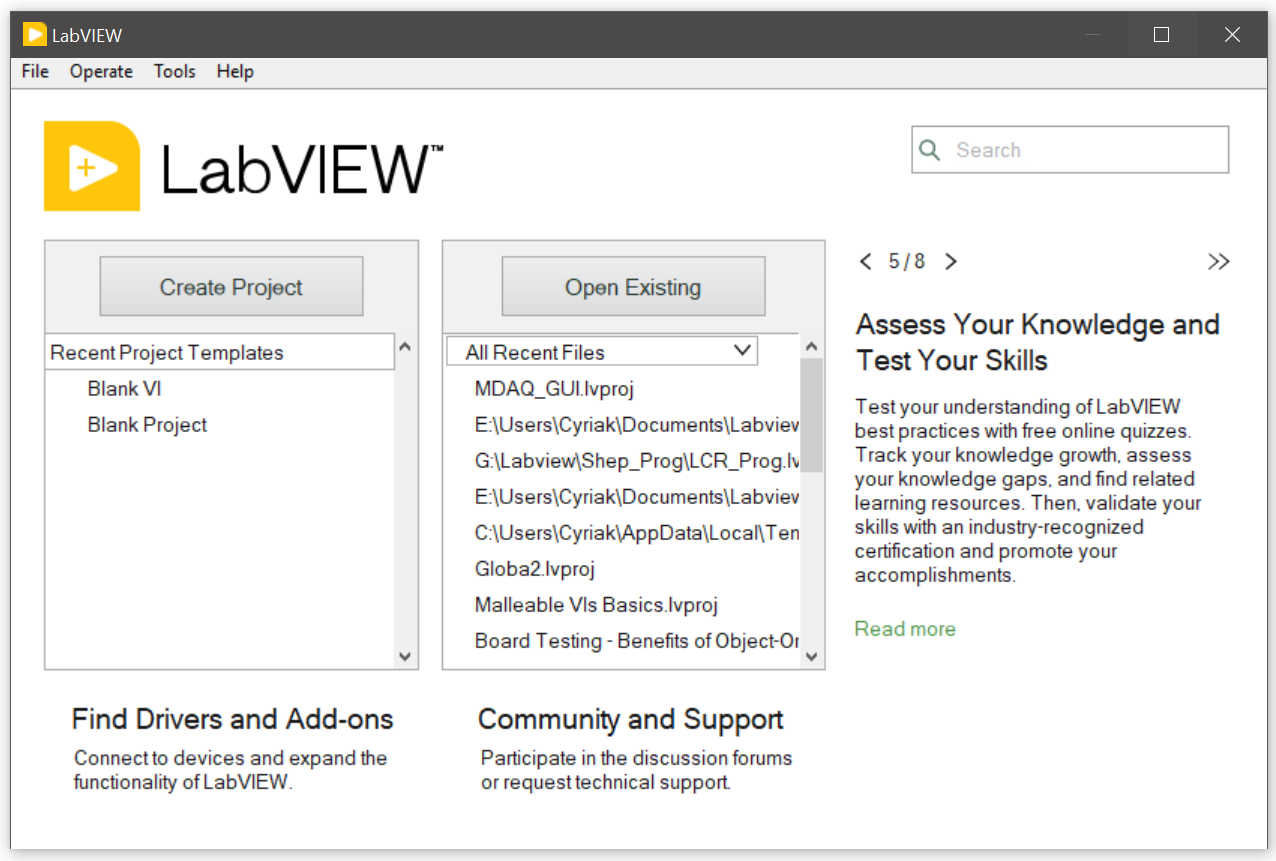
\includegraphics[width=\textwidth]{startup}
		\caption{The window $\labview$ greats you with on startup.}
		\label{startup}
	\end{figure}

	Two windows will pop up, a ``Front Panel'' and a ``Block Diagram''. You will need to familiarise yourself with the $\labview$ interface, this is best done by exploration, trail and error. Simply mousing over any button should give you some clue as to what the button does or what is contained in the menus. You probably would not break your computer or the $\labview$ installation by playing around with the interface.\\
	
	In the next few sections we will go over what is meant by a VI, the difference between the block diagram and the front panel,
	how to cycle between these views, and how to place objects on these windows.
	
	\subsection{The VI}
	As stated before, VI is short for virtual instrument. The idea is that you create an interface which may be operated by a human, usually with a mouse and keyboard. This interface is called the ``Front Panel'' in $\labview$. You then glue the elements of the front panel together in the ``Block Diagram'', this is where the $\labview$ magic happens, or the $\labview$ logic execution engine, if you do not believe in magic.\\
	
	Figure \ref{exampleFront1}, on page \pageref{exampleFront1}, shows one of the first front panels I have ever created along with the block diagram in figure \ref{exampleBlock1}. By the end of this course you will be able to understand exactly what is going on there so do not let it intimidate you. Assert dominance over your computer, lest it assert dominance over you. %TODO Maybe make this a CS Lesson?
			\begin{figure}
			\centering
			\begin{subfigure}[b]{0.49\textwidth}
				\centering
				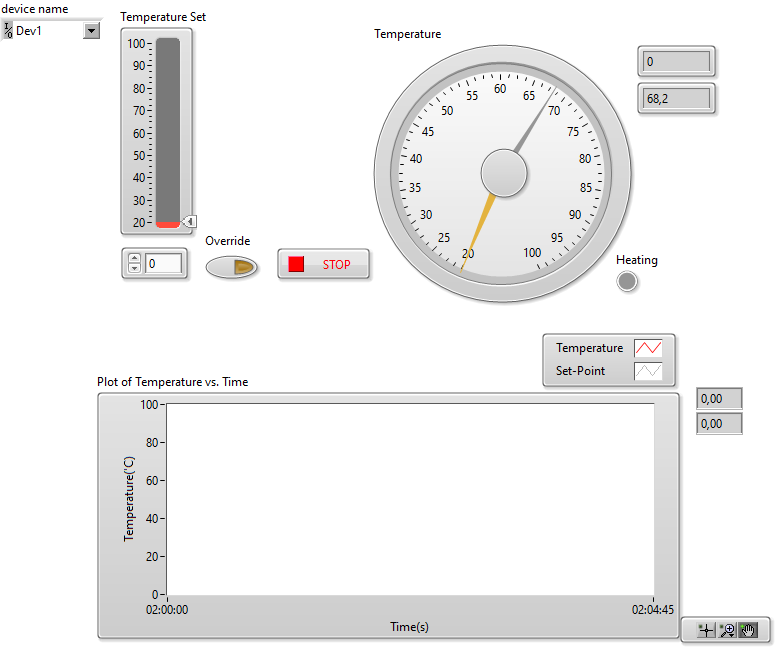
\includegraphics[width=\textwidth]{exampleFront1}
				\caption{A more useful front panel.}
				\label{exampleFront1}
			\end{subfigure}
			\hfill
			\begin{subfigure}[b]{0.49\textwidth}
				\centering
				\includegraphics[width=\textwidth]{ExampleBlock1}
				\caption{The logic behind the front panel.}
				\label{exampleBlock1}
			\end{subfigure}
			\caption{A program which turns a kettle on and off to achieve a set temperature.}
			\label{oldExample}
		\end{figure}
	\subsubsection{The Front Panel}
	Figure \ref{EmptyFront} shows an empty front panel. \texttt{Right click}ing anywhere on the grey grid will open a menu containing controls, known as the ``controls palette''. Do not be overwhelmed, given some time you will get a feel for where the most important controls are. As mentioned, and will be repeated throughout this book, explore the interface on your own.\\
	\begin{figure}
		\centering
		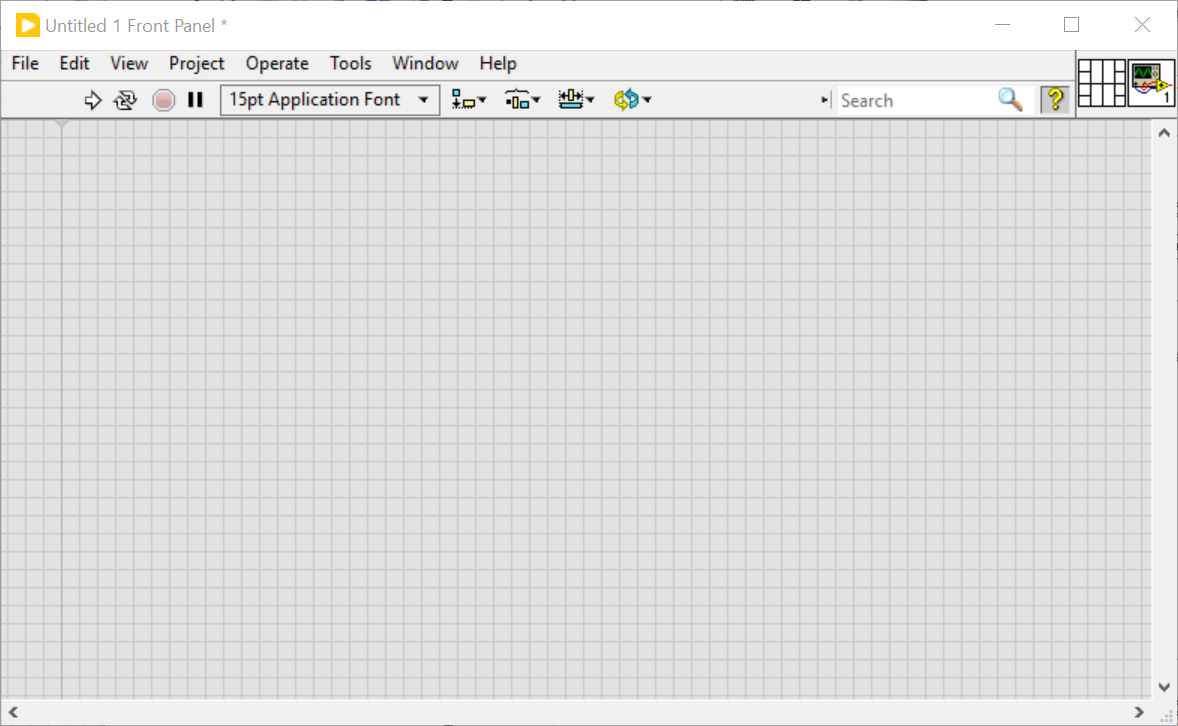
\includegraphics[width=\textwidth]{EmptyFront}
		\caption{A barren wasteland of a front panel, not very useful.}
		\label{EmptyFront}
	\end{figure}

	Here is a little secret, simply press \texttt{Ctrl+H}. This will open a floating window called ``Context Help'', your new life-line in $\labview$. Hover over anything and it will give you some information about what you are looking at.  Pressing ``Detailed help'' takes you to the $\labview$ help files. You will spend a great deal of time reading these documents as you progress through your $\labview$ journey so you should know where to find it.\\
	
	If you figured out how to place down controls in $\labview$, that is great, do not let the interface intimidate you. If you have not done so yet, we will go through the details in section \ref{HowToPlace}.
	\subsubsection{The Block Diagram}
	The sibling panel to figure \ref{EmptyFront} may be found in figure \ref{EmptyBlock}. As before, you may \texttt{Right click} on the white background to open the ``functions palette''. This is where you will spend most of your time in $\labview$, other than the help files that is. You thread together small function blocks to build the logic of your program. If you are reading this and can't find the block diagram panel, simply press \texttt{Ctrl-E}, this will switch from the front panel to the block diagram and vice versa. This is probably the most important hot-key in $\labview$ so learn it, you will often have to flip between the two windows.\\
	\begin{figure}
		\centering
		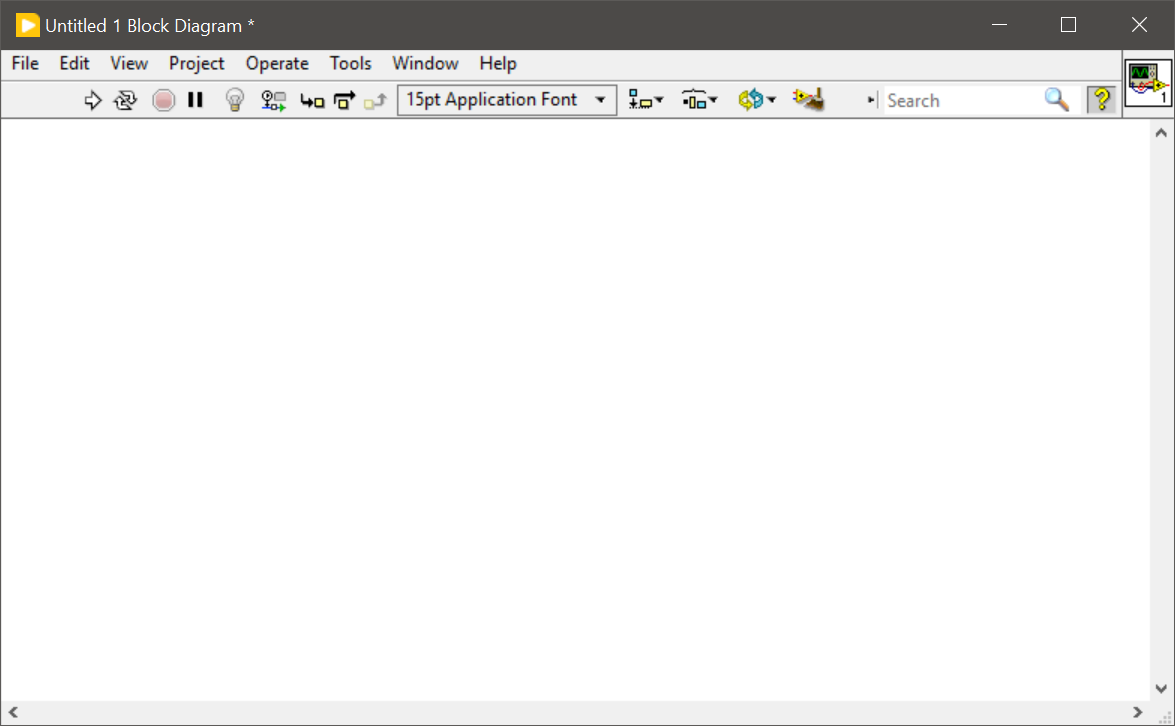
\includegraphics[width=\textwidth]{EmptyBlock}
		\caption{The void, even interstellar space has more going on than this panel.}
		\label{EmptyBlock}
	\end{figure}

	\section{LabVIEW variables and you}
	\subsection{Overview}
	From your knowlage of mathematics, you understand the concept of a variable. This concept is of fundamental importance to all fields of computer science so let us take a slight detour before we dig further into $\labview$.\\
	
	Variables are named containers in which we may store information. It is then possible to read from, or write to, this container using it's name. At any moment in time, there are several named variables in your head, for example: \texttt{cellphoneNumber, currentDate, amountOfCoffeeHadToday,} etc.\\
	
	With these examples, it is clear that some variables are not of the same type, i.e. saying ``I had 3 June 2022 coffees today'' makes no sense. You should know by now, or if you do not you will learn very soon, that computers are incredibly stupid and they will happily add 3 June 2022 to 072 543 7711 and give you a result. (The answer is 29 May 2045 by the way).\\
	
	In general, it is your job to tell the computer what type a variable is. This is not strictly true as many programming languages can infer the data type from your input, however for $\labview$ and programming languages such as \texttt{C} and \texttt{C++}, you are responsible.
	
	\subsection{Variable Types}
	\subsubsection{Boolean}
	Perhaps the most fundamental variable type is the boolean, or bool for short. It consists of either yes or no, true or false, \texttt{1} or \texttt{0}, you get the picture. In $\labview$, bools form the basis of nearly all your decision making code. It is represented as green icons, seen in figure \ref{boolFig}, on page \pageref{boolFig}.
	\subsubsection{Floating Point}
	Floating point variables hold decimal numbers, in an application this may be the value of a magnetic field, the temperature of a thermocouple, basically any number that you can think of that would fit into 64bits of memory (more on that if you do computational physics in honours physics). All floating point values are represented in Labview as orange icons, seen in figure \ref{floatFig}, on page \pageref{floatFig}.
	\subsubsection{Integer}
	The integer type is self explanatory. This is the only type of number which may be represented in $\labview$ as exact numbers and is ideal for comparison and counting. It is worth mentioning briefly that integers exist as two types namely signed and unsigned. Negative numbers are contained in signed integers, unsigned integers are strictly positive. The nuances of signedness are best left for the computational physics coarse in honours. Integer types are represented as blue icons in $\labview$, see figure \ref{intFig} on page \pageref{intFig}.
	\subsubsection{Strings}
	This line that you are reading is a string. Strings are made up of characters, itself a type of variable. Characters are not as important in $\labview$ as in other programming languages so they do not deserve their own subsection. Strings may be used to convey information to users, it may also be used to store information on your hard-disk. Strings are pink in $\labview$, reference \ref{stringFig} on page \pageref{stringFig}.
	\subsubsection{Arrays}
	\label{ch1Arrays}
	Arrays are homogenous sections of sequential memory. Any of the above data types may be formed into an array. This variable type allows you to reference a collection of data points as a single item. Unless you derive joy from naming thousands of individual variables, you should use arrays when working with more than a handful of data points. Arrays are indexed from 0 in $\labview$, important if you have programmed in Fortran before. Arrays follow the colour of their contents in $\labview$, i.e. a blue array contains only integers.
	\subsubsection{Aggregate Types}
	Variable types may be grouped together to form a new variable type, usually with some relationship among one another. In $\labview$, these types are known as clusters, similar to structs from the \texttt{C} family of languages. We will leave clusters for now, they are only really useful once your programs start getting big.
	\begin{figure}
		\centering
		\begin{subfigure}[b]{0.49\textwidth}
			\centering
			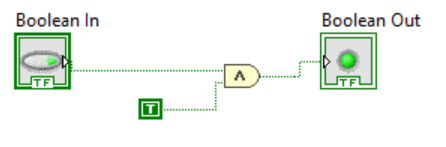
\includegraphics[width=\textwidth]{boolFig}
			\caption{Boolean controls and constants.}
			\label{boolFig}
		\end{subfigure}
		\hfill
		\begin{subfigure}[b]{0.49\textwidth}
			\centering
			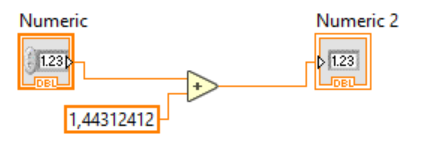
\includegraphics[width=\textwidth]{floatFig}
			\caption{Floating point controls and constants.}
			\label{floatFig}
		\end{subfigure}
		\vfill
		\begin{subfigure}[b]{0.49\textwidth}
			\centering
			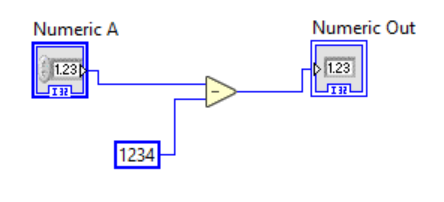
\includegraphics[width=\textwidth]{intFig}
			\caption{Integer data types.}
			\label{intFig}
		\end{subfigure}
		\hfill
		\begin{subfigure}[b]{0.49\textwidth}
			\centering
			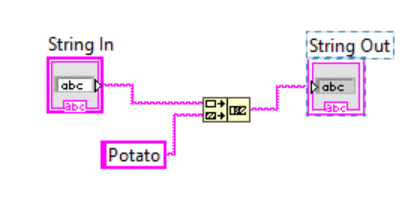
\includegraphics[width=\textwidth]{stringFig}
			\caption{String data types}
			\label{stringFig}
		\end{subfigure}
		\caption{Fundamental $\labview$ data types.}
		\label{DataTypes}
	\end{figure}
	
	\section{Your First LabVIEW program}
	\subsection{Problem statement}
	We must create a program in which a user gives three integer values, \texttt{numberA}, \texttt{numberB}, and \texttt{NumberC}. The program needs to compute and output the sum of \texttt{numberA} and \texttt{numberB} as well as indicate if this sum is larger than \texttt{numberC}.\\
	
	The rest of this section will show you in detail how such a program is made in $\labview$, however it will not explain the details of the program in depth. This is left for later sections in chapter 2.\\%TODO reference chapter
	\subsection{Implimentation}
	\subsubsection{Front Panel}
	\label{HowToPlace}
	You may think of the front panel as your scratch pad. What information does the user need to provide for our program and how may the computer display the outcome of a process?\\
	
	Anywhere on the front panel, \texttt{right click} to show the control palette. Mouse over the top left folder called ``Numeric'', a new window will pop up. Drag your mouse into this window and select ``Numeric Control'' by clicking once on the icon. You will notice that your mouse cursor now changed to a little grab hand with an outline of the proposed control. Simply click where you would like this control to live.\\
	
	The name ``Numeric'' is not helpful to us. If the name is highlighted, white text in a black box, you may type a new name and it would replace the old one. Call this control ``numberA''. If the name is not highlighted, simply \texttt{double click} on the name until you see the black box with white text and then type ``numberA''. Once you have typed the name, \texttt{left click} anywhere on the background to make the change permanent.\\
	
	Figure \ref{blackboxtext} shows how selected text looks like and what you should have on your front panel after you have renamed the control. Repeat what you have just done two more times to create ``numberB'' and ``numberC''.\\
	\begin{figure}
		\centering
		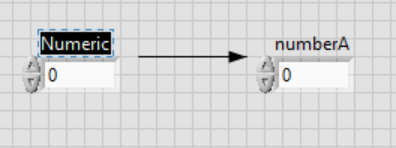
\includegraphics[width=0.5\textwidth]{blackboxtext}
		\caption{What you should have after renaming the control.}
		\label{blackboxtext}
	\end{figure}
	
	For our resulting number, open the controls palette, go to ``Numeric'' and select the ``Numeric Indicator'' icon. Rename this to ``Result''.\\
	
	Finally, open the control palette again, this time go to the ``Boolean'' folder and select the ``Round LED''. You should place this close to your result indicator. You will start to notice that grouping controls together with regards to input and output makes it easier to understand the intent of your program. Lastly, rename this indicator to ``Result is greater than numberC?''.\\
	
	Your front panel should now look like the panel in figure \ref{example1Front} on page \pageref{example1Front}.\\
	\begin{figure}
		\centering
		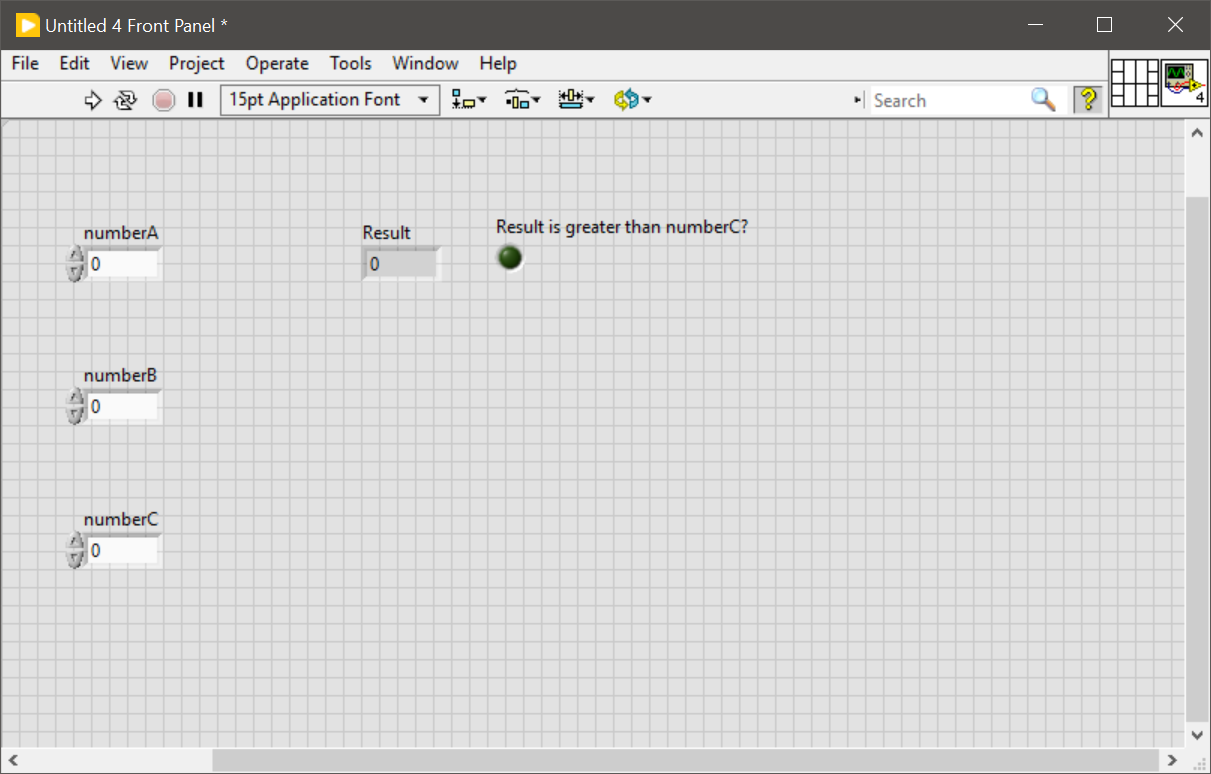
\includegraphics[width=\textwidth]{example1Front}
		\caption{Roughly what your front panel should look like..}
		\label{example1Front}
	\end{figure}
	
	If you are not satisfied with your layout, you may \texttt{left click} and hold on the edges of a control and drag it to where you would like to to be. This might take some getting used too. Your cursor will change from a cross to a pointer when you hover over a part of a control which is allowed to be moved. %TODO This is not writen well I know
	\subsubsection{Block Diagram}
	While looking at your front panel, press \texttt{Ctrl-E} to flip to your block diagram. You would notice that what you have done on the front panel is reflected in the block diagram. Your inputs have little white arrows pointing out of the icon to the right. The outputs, also known as indicators in $\labview$, have white arrows pointing into the icon on the left.\\
	
	You should move these icons so that the interface flows from left to right, that is, inputs on the left and outputs on the right. You move the icons like you have moved the front panel elements, just click, hold, and drag the icons to where you think they should live. See figure \ref{example1Block} for inspiration.\\
	\begin{figure}
		\centering
		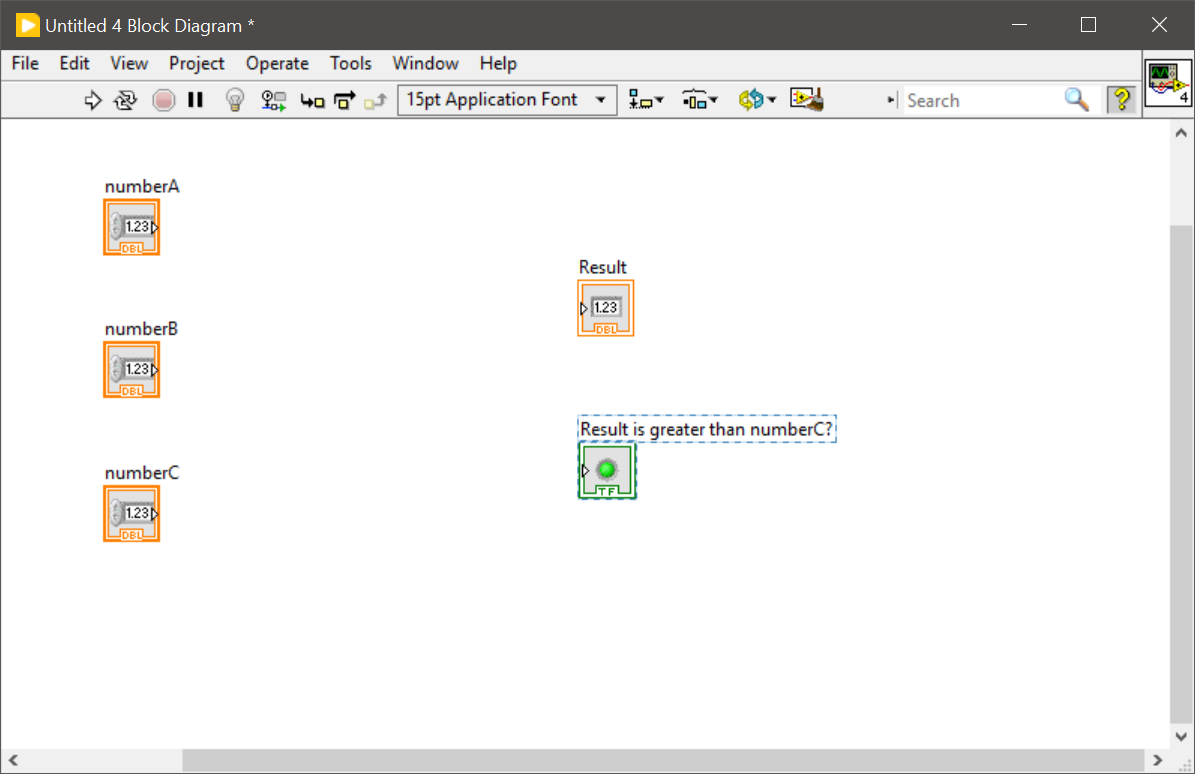
\includegraphics[width=\textwidth]{example1Block}
		\caption{More or less what your block diagram should look like.}
		\label{example1Block}
	\end{figure}

	You are now ready to build the logic of your program. From our problem statement, we need to sum numberA and numberB. Both are numerical values so we go to the ``Numeric'' folder of the function palette. The first icon you see is the add function. Place it somewhere in the middle of your inputs and outputs.\\
	
	Hover your mouse cursor over the newly placed function, you will notice that little orange terminals are highlighted. If you hover over one of your number inputs, you will also see a little terminal, conveniently placed next to the white arrow. \texttt{Left click} on the terminal of numberA, moving your mouse around the screen you will see a black striped line following your cursor. Then \texttt{left click} on one of the terminals of the add function. You would see something like figure \ref{wireinprogress} before you click. This will create an orange line, also known as a wire, connecting your input to the function.\\
	\begin{figure}
		\centering
		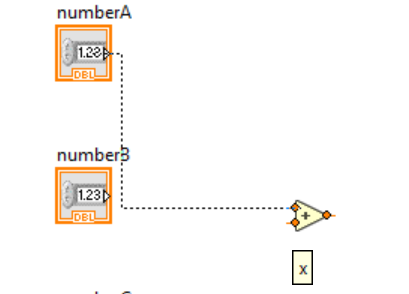
\includegraphics[width=0.5\textwidth]{wireinprogress}
		\caption{A ghostly wire follows your cursor to your desired terminal.}
		\label{wireinprogress}
	\end{figure}

	Connect numberB to the add function, then connect the output of the add function to the result indicator. You should now have a block diagram that looks like figure \ref{example2Block} on page \pageref{example2Block}.\\
		\begin{figure}
		\centering
		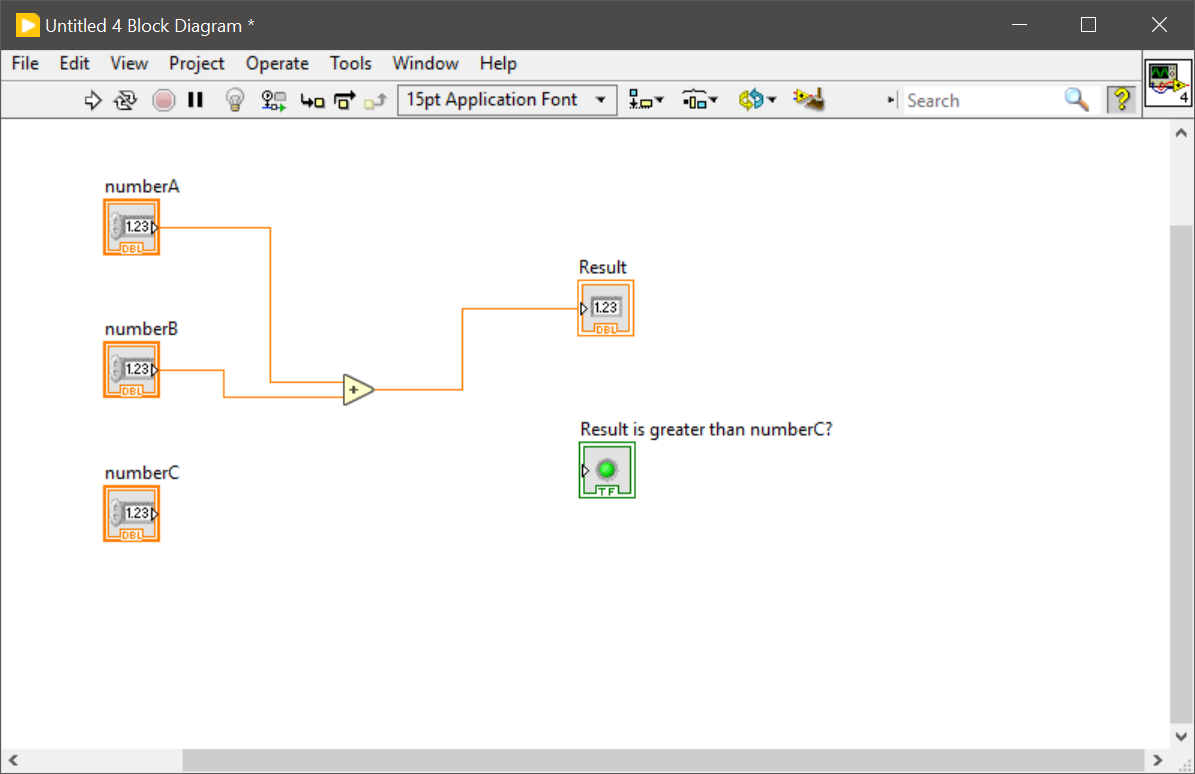
\includegraphics[width=\textwidth]{example2Block}
		\caption{The summing logic wired correctly, your block diagram should look like this.}
		\label{example2Block}
	\end{figure}

	From the function palette, select the ``comparison'' folder and look for the function that says ``greater than''. It is the triangle with the > symbol on it. Place this somewhere below the add function, but still between the controls and the indicators.\\
	
	You should now wire the output from this function to the terminal of your LED. The function compares two inputs and sends a true value to the LED if the one input is greater than the other, but how do we know which input is which? The ``context help'' window will show you which input is which, see figure \ref{context1Help}. If you do not see this window, just press \texttt{Ctrl+H} on your keyboard.\\
	\begin{figure}
		\centering
		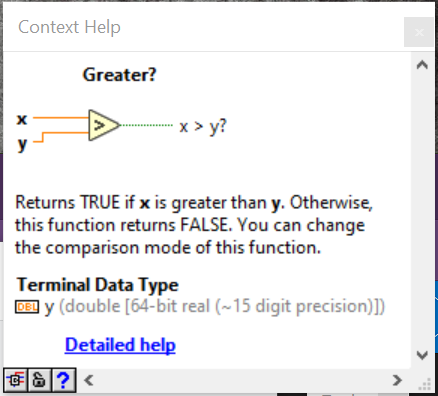
\includegraphics[width=0.5\textwidth]{context1Help}
		\caption{The context help for the comparison function, the top terminal is $x$ and the bottom one is $y$.}
		\label{context1Help}
	\end{figure}
	
	Wire in the value from numberC into the comparison function and connect the other input to the output of your summing function. You may do this by starting the wire at the input of the comparison function and \texttt{Left clicking} on the wire leading from the summing function to your result indicator. It is also possible to \texttt{Right click} on the wire leading from the summing function and selecting the ``Create wire branch'' option from the menu. You then wire this into the comparison function.\\
	
	Finally, your block diagram should look like the one in figure \ref{example3Block}. You may also move around the wire pieces by \texttt{left click}ing on them and dragging them about.\\
	\begin{figure}
		\centering
		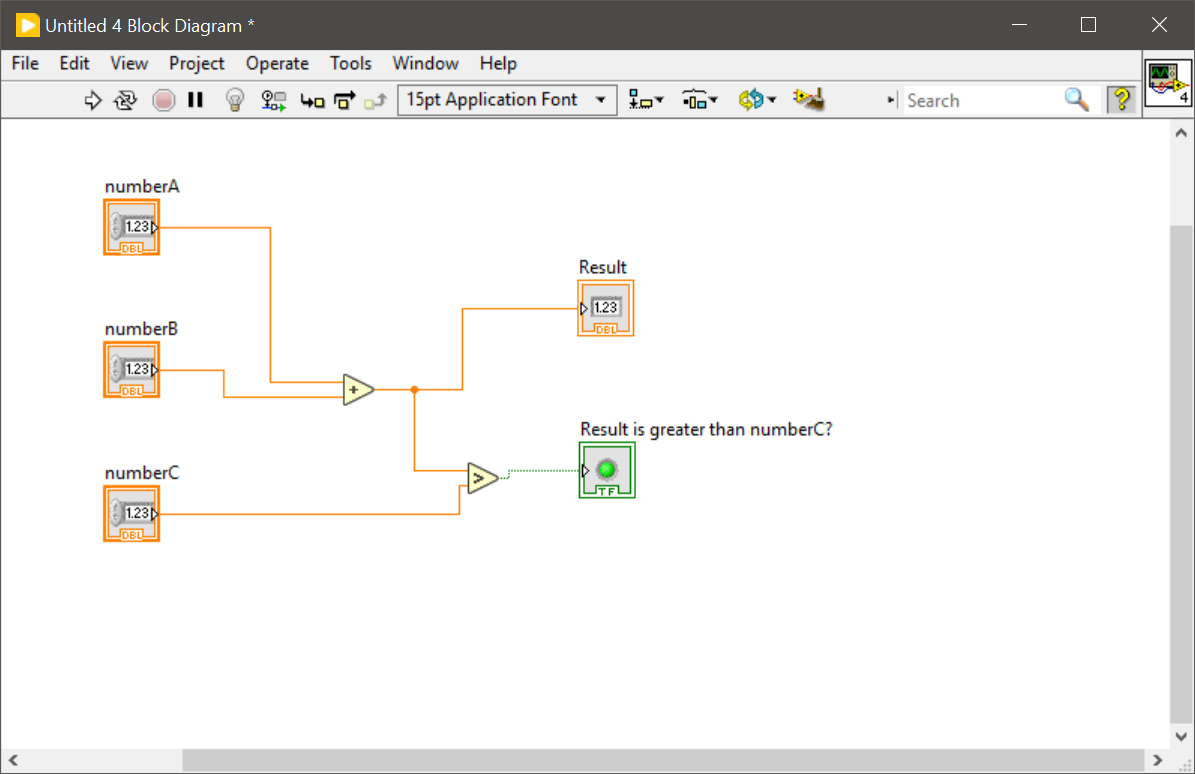
\includegraphics[width=\textwidth]{example3Block}
		\caption{The final wired block diagram.}
		\label{example3Block}
	\end{figure}

	\subsection{Testing your program}
	You may now go back to your front panel. You can click in the centre of the controls and type in a value. Do this for all three number controls and press the play button, the one found near the top left of your window.\\
	
	Does your results make sense? Is the summing correct? Is the light on? Should it be on? These are all the questions that you should have when testing your program. Figure \ref{exampleFrontTrue} shows what happens when the sum of numberA and numberB is greater than numberC. Figure \ref{exampleFrontFalse} shows when numberC is smaller than the sum. If your program does the opposite of what it is supposed to do, make sure that you have wired in the correct terminals and have selected the correct comparison function. It is worth noting that the VI executes once and stops. After you have typed in new values, you will need to run the VI again.\\
	\begin{figure}
		\centering
		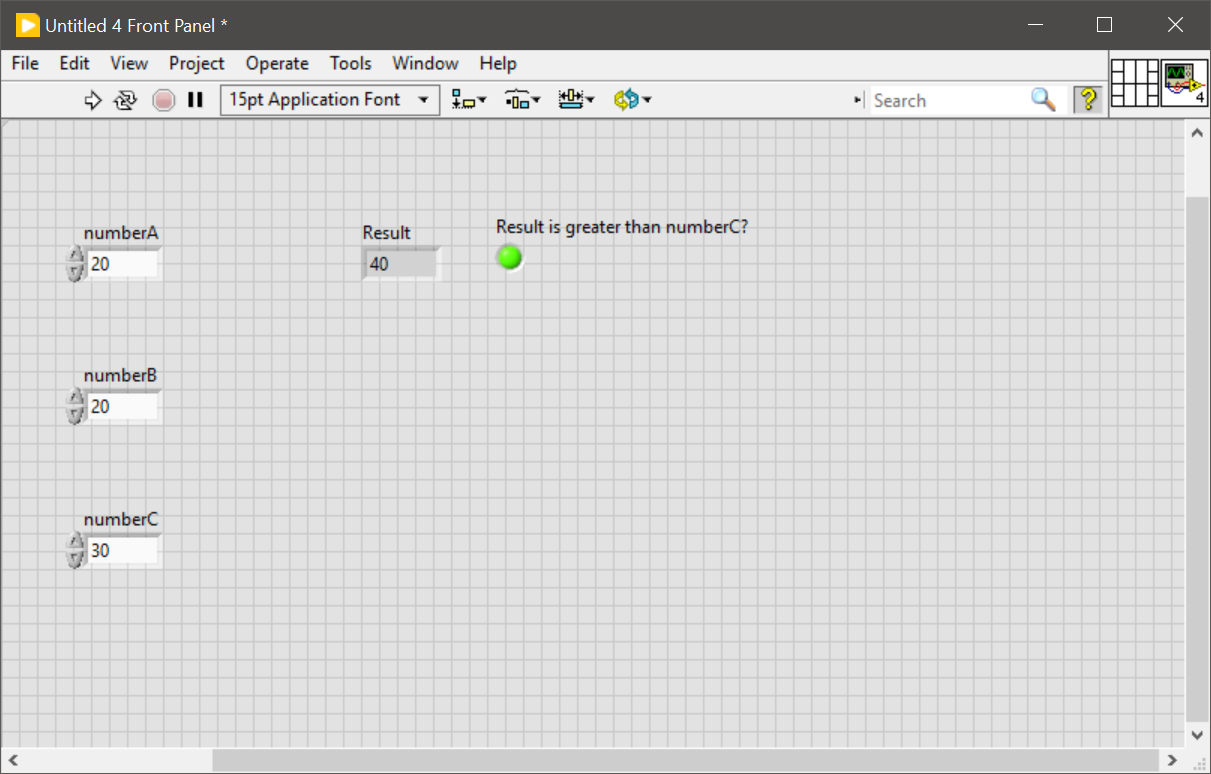
\includegraphics[width=\textwidth]{exampleFrontTrue}
		\caption{The sum is 40 which is greater than 30 so the LED is on.}
		\label{exampleFrontTrue}
	\end{figure}
	\begin{figure}
		\centering
		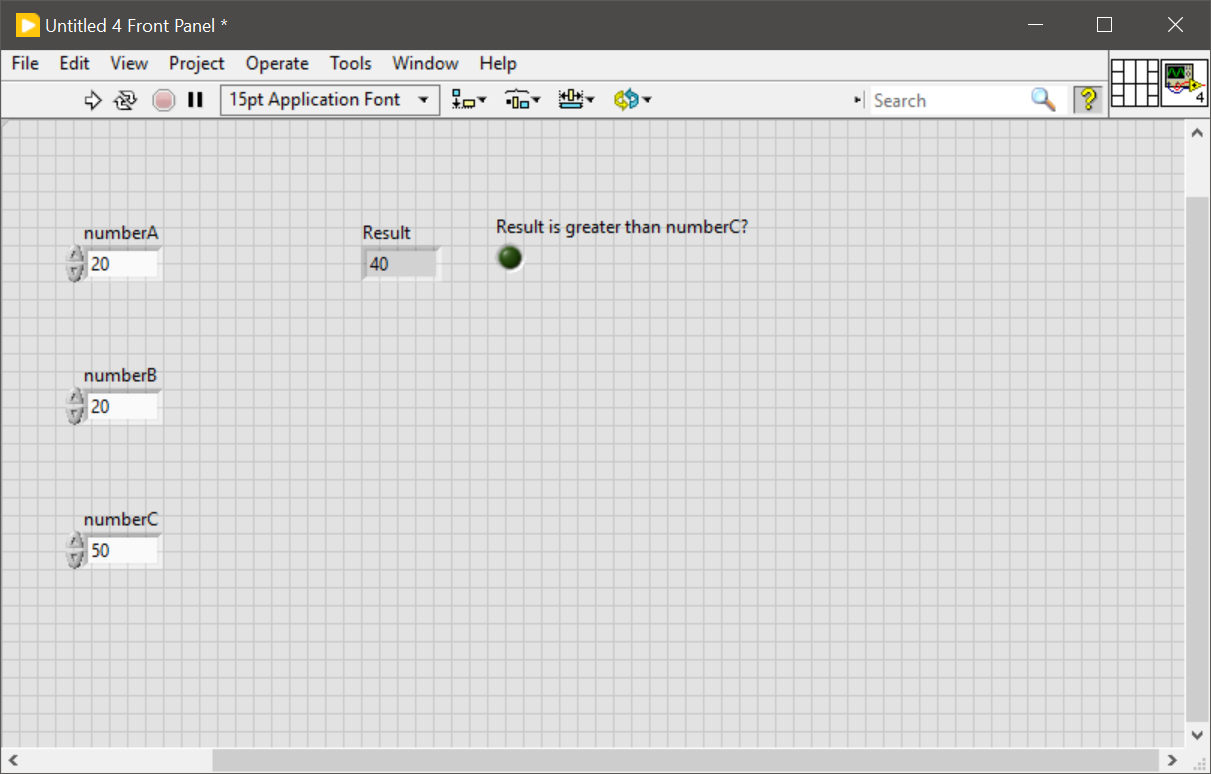
\includegraphics[width=\textwidth]{exampleFrontFalse}
		\caption{Changing numberC to 50 turns the LED off.}
		\label{exampleFrontFalse}
	\end{figure}

	You may now save your VI by clicking ``File'' on the task bar and selecting save from the menu. Name it something like ``helloworld.vi''.
	
	\subsection{Review}
	From this example, you have learned how to open $\labview$ and how to create a VI. You have also learned how programs are built using the front panel and the block diagram. This is enough for you to start experimenting with the available functions to create interesting programs.
	
	\subsection{A word on Accessibility}
	\subsubsection{Colour Blindness}
	You may have noticed the unique colours attributed to different variable types, if you didn't, you may be colour blind. As of Q3 2022, $\labview$ has no colour-blind friendly mode so you need to study figure \ref{DataTypes}, on page \pageref{DataTypes}, and make a note of the colours you struggle to distinguish. The icons also provide small abbreviations, i.e.  \textsc{tf} for boolean and \textsc{dbl} for floating point types.\\
	
	If this is not useful to you, you may change the colour filter on your computer if you are a windows user. Go to: Start\textgreater Settings\textgreater Ease of Access. Then select the Colour filters option. Here you will be able to change the colour profile of your monitor, do this while having an example VI open until you can distinguish the variable types with ease.
	\subsubsection{Vision Difficulty}
	Depending on various factors, you my struggle to build a block diagram in $\labview$ due to everything being small. As of Q3 2022, $\labview$ still does not offer a zoom feature for you to connect terminals easier. A workaround for this is to use the UI scaling feature built into windows.\\
	Go to: Start\textgreater Settings\textgreater Ease of Access. Then select the display option. Here you may scale the UI using the ``Make everything bigger'' option. Adjust this value until you are comfortable connecting terminals in $\labview$.
	
	\pagebreak
	\section{Mini Projects}
	\begin{enumerate}
		\item You are building a safety interlock system for your laboratory.\\
		A powerful x-ray source is required to perform diffraction measurements on powdered samples. This x-ray source requires water to flow through its manifold so that it does not overheat and burnout. If this breaks, you owe the laboratory R100 000 in repair fees. Although the x-rays you receive at the dentist is safe, the intensity of the x-rays used for XRD would cause serious radiation burns which could lead to cancer, the x-ray source should not be allowed to run if the safety door is open.\\
		
		Build a interlock system in $\labview$ that would prevent damage to the XRD machine and prevent damage to you.\\
		
		To achieve this, you may use switches on your front panel to indicate whether water is flowing through the system and whether the safety door is closed or not. You need a switch that would be the power switch for the x-ray source. Your program needs to light up an LED indicator if the power is switched on and the conditions for operation are met. If the conditions are not met, the LED indicator should not light up.
		
		\item You have a few friends from the United States who do not understand the Celsius temperature scale.\\
		They are confused that we are walking around on the beach when it is 30\textdegree outside.\\
		
		Build a simple program which would accept a numerical input as degrees Celsius and convert that to Fahrenheit. This should allow your friends to get a feel for the Celsius temperature scale.\\
		
		This program is rather boring, let us make it more interesting by adding indicator lights for the boiling point and freezing point for a couple of materials. For example, if the input temperature is 50\textdegree, neither the boiling nor the freezing light should be on. If the temperature is above 100\textdegree, the boiling light should be on. You should have lights for water and ethanol. Bonus marks for an extra substance.\\
	\end{enumerate}
	
	